\subsection{Исследование профиля высвечивания сместителя спектра}\label{section:secWLS}

Анализ распределения во времени хитов, принадлежащих одному черенковскому кольцу, позволяет исследовать временные свойства сместителя спектра. Анализу подлежит распределение разностей временных отметок хитов каждого кольца относительно первого по времени хита в данном кольце. В зависимости от длины волны черенковский фотон может с той или иной вероятностью либо поглотиться сместителем спектра и вызвать его свечение, либо пройти сквозь слой сместителя спектра без взаимодействия и попасть фотокатод. В результате, даже при наличии слоя сместителя спектра, часть хитов подчиняется временной зависимости характерной для чистого ФЭУ. Таким образом, для получения кривой высвечивания сместителя спектра необходимо из распределения разностей времен, полученного со сместителем спектра, вычесть должным образом отнормированное в максимуме распределение разностей времён, полученное с чистым ФЭУ.

Нормированные в максимуме кривые высвечивания со сместителем спектра и без него показаны на \figref{fig:WLStwoCurves}, а разность этих распределений --- на \figref{fig:WLSdiff}. Видно, что за исключением небольшой выпуклости в области 7~нс, связанной с особенностями работы данного семейства МА~ФЭУ, кривая выглядит похоже на сумму нескольких экспонент.

\begin{figure}[H]
\centering
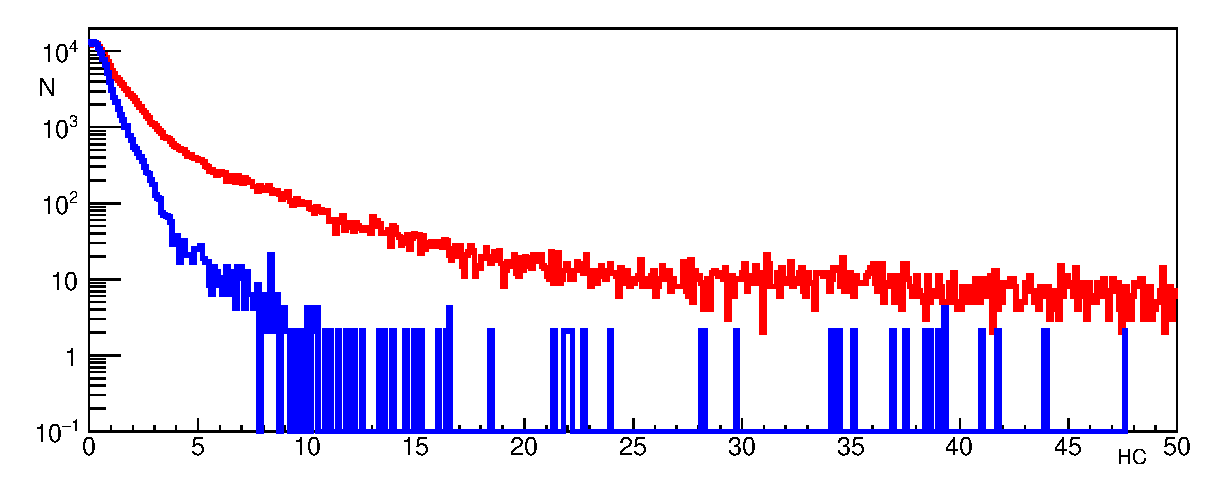
\includegraphics[width=1.0\textwidth]{pictures/26_WLS_8feb.eps}
\caption{Измеренные распределения, соответствующие кривым высвечивания со сместителем спектра (красный, выше) и без него (синий, ниже).}
\label{fig:WLStwoCurves}
\end{figure}

\begin{figure}[H]
\centering
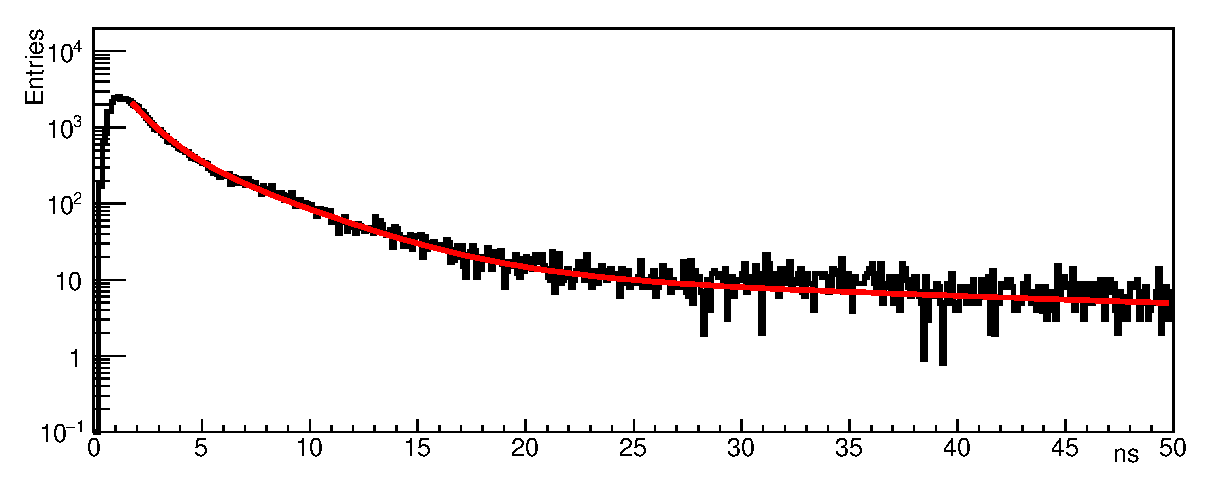
\includegraphics[width=1.0\textwidth]{pictures/27_WLSdiff_8feb.eps}
\caption{Разница распределений со сместителем спектра и без него и кривая --- результат фитирования распределения суммой трёх экспонент.}
\label{fig:WLSdiff}
\end{figure}

Указанная выпуклость не позволяет надёжно извлечь характерные времена высвечивания. Интересно, тем не менее, сравнить полученную кривую с результатами флюориметрических исследований. Стеклянная пластина со слоем сместителя спектра, нанесённым точно таким же методом, как и на МА~ФЭУ, была исследована с помощью классического метода счёта фотонов при возбуждении светом с длиной волны 280~нм~\cite{DUERR}. Были получены значения времён высвечивания 1.4~нс, 3.8~нс, и 45~нс и соответствующие относительные интенсивности компонент 1.8996, 1.0000, и 0.8364.

% УКАЗАТЬ ИНТЕГРАЛЫ, НОРМИРОВАННЫЕ ТАК, ЧТО 3.8 нс СООТВЕТСТВУЕТ 1.

% Мы выяснили, что эти значения - это амплитуды. Следовательно их нужно домножить на соответствующие времена
% 1387, 269, 19
% 1387*1.4 = 1941.8
% 269*3.8 = 1022.2
% 19*45 = 855

% Затем нормируем по второй компоненте и получаем
% 1.8996
% 1.0000
% 0.8364

Подгонка кривой с \figref{fig:WLSdiff} суммой трех экспонент с соответствующими временами показывает разумное согласие для времен превышающих 5~нс. Начальный участок лучше подгоняется с характерным временем $\tau_{1}$=1.1~нс. Сравнение интенсивностей наиболее быстрой компоненты с флюорометрическими измерениями затруднено из-за начального неэкспоненциального участка, а относительный вклад наиболее медленной компоненты в полную интенсивность в нашем случае оказывается в 3.8~раз ниже. Это можно объяснить влиянием способа возбуждения на заселение разных типов центров высвечивания.

В пределе большого числа хитов в кольце использованный нами метод переходит в стандартный метод исследования флюоресценции путем счета единичных фотонов~\cite{SPC}. Однако в нашем случае существует некоторая случайная задержка между моментом попадания черенковского фотона на поверхность МА~ФЭУ и временем прихода первого хита. С целью выявления влияния метода на измеренные времена высвечивания было проведено Монте Карло моделирование.

В модели были заложены разброс времени прохода лавины в МА~ФЭУ 300~пс (RMS), три экспоненциальные компоненты с характерными временами 1.4~нс, 3.8~нс, и 45~нс и относительными интенсивностями 2.17, 1.00, 0.22 и средним числом хитов в кольце равным~18. Получившееся распределение времён односительно первого хита в кольце было подогнано трёмя экспонентами со свободными параметрами. Если начать фитирование получившейся зависимости, отступив 4~нс от начала высвечивания, величины постоянных распада экспонент воспроизводятся с точностью лучше 5\%, а соответствующие относительные интенсивности несколько искажаются, что естественно, в силу существования начального неэкспоненциального участка кривой. Таким образом, подтверждена корректность применённого метода определения времён высвечивания.

Практическая ценность проведенного исследования состоит в том, что может быть оптимизирована длительность окна, в пределах которого хиты принимаются одновременными и могут быть приписаны одному событию. Для этого необходимо найти баланс между числом дополнительных хитов, полученных благодаря сместителю спектра и вероятностью наложения сигналов друг на друга или подхвата в кольцо темнового хита. Например, прирост хитов в 19\% может быть достигнут при длительности окна 15~нс.

% Принимаем, что во всём диапазоне (50 нс) прирост хитов навен 21% (инфа извне).
% Всего в гистограмме WLS_diff в интервале 50 нс 72609 вхождений.
% 21% = 72609
% 100% = 345757
% 121% = 72609+345757 = 418366
% В диапазоне 0-15 нс интеграл равен 68220.
% 68220/345757 = 19.73%
% 68220/72609 = 94%
% 94% от 21(%) = 19.74(%) Такие дела.
